\documentclass[11pt,a4paper]{article}

\usepackage[T1]{fontenc}
\usepackage{lmodern}
\usepackage[margin=2.3cm]{geometry}
\usepackage{amsmath,amssymb}
\usepackage{graphicx}
\usepackage{booktabs}
\usepackage[font=small,labelfont=bf]{caption}
\usepackage{xcolor}
\usepackage[colorlinks=true,linkcolor=blue!50!black,citecolor=blue!50!black,urlcolor=blue!50!black]{hyperref}

\graphicspath{{figures/}}

\newcommand{\Jw}{J_{\mathrm{w}}}
\newcommand{\Js}{J_{\mathrm{s}}}
\newcommand{\dg}{^{\dagger}}

\title{Can a topological edge survive strong interactions?}
\author{\textit{[your name]}}
\date{QFT course project (Project A), 2026}

\begin{document}
\maketitle

%======================================================================
\section{Model}
\label{sec:model}

We study spinless fermions on an open chain of $L$ (even) sites $j=0,\dots,L-1$ at half filling, $N=L/2$:
\begin{equation}
  H = -\sum_{j=0}^{L-2} J_j \left(c_j\dg c_{j+1} + \text{h.c.}\right)
      + V \sum_{j=0}^{L-2} \left(n_j - \tfrac12\right)\left(n_{j+1} - \tfrac12\right),
  \qquad J_j = 1 + (-1)^j \delta .
  \label{eq:H}
\end{equation}
The hopping alternates between weak and strong bonds (the SSH chain), and $V$ is a nearest-neighbour repulsion.
We set $\hbar = J = 1$.
For $\delta<0$ the chain starts and ends on a weak bond, $J_0 = J_{L-2} = \Jw = 1-|\delta|$; the strong bond is $\Js = 1+|\delta|$, and $r = \Jw/\Js$.
We ask how the localisation, spectral weight and entanglement of the edge excitation change as $V$ increases.

%======================================================================
\section{Step 1: the free edge problem}
\label{sec:step1}

\subsection{What was done}

At $V=0$ the problem reduces to the $L\times L$ hopping matrix $h_{j,j+1} = h_{j+1,j} = -J_j$.
We diagonalised it for $L\in\{40,80,120\}$ and $\delta\in\{\pm0.15,\pm0.30,\pm0.50\}$, and compared the results with the analytic edge state derived below.

\paragraph{Edge wavefunction.}
Hopping only connects even sites to odd sites, so a zero-energy state can be sought on the even sites alone.
Take a semi-infinite chain, $j\ge0$, with $\delta<0$, so $J_{2\ell}=\Jw$ and $J_{2\ell+1}=\Js$.
With $\psi_{2\ell+1}=0$, the rows of $h\psi=0$ at even sites hold automatically.
The row at site $2\ell+1$ gives $\Jw\psi_{2\ell}+\Js\psi_{2\ell+2}=0$, so $\psi_{2\ell}=\psi_0(-r)^\ell$.
Normalising with $\sum_\ell r^{2\ell}=1/(1-r^2)$ gives
\begin{equation}
  \psi_{2\ell} = \sqrt{1-r^2}\,(-r)^\ell,\quad \psi_{2\ell+1}=0,
  \qquad |\psi_j|^2 = (1-r^2)\,e^{-2j/\xi},\qquad \xi = \frac{2}{\ln(\Js/\Jw)} \simeq \frac{1}{|\delta|}.
  \label{eq:xi}
\end{equation}
The amplitude falls by $r$ per two-site cell, which is the origin of the factor 2 in $\xi$.
For $\delta>0$ the same recursion gives $\psi_{2\ell}\propto(-1/r)^\ell$, which cannot be normalised, so there is no zero mode at a strong end bond.
On a finite chain the two states nearest $E=0$ are spread over both ends.
To isolate the left-edge state we diagonalised the position operator $X$ within their two-dimensional subspace.
As an independent check, we also diagonalised the chiral operator $\Gamma=\mathrm{diag}((-1)^j)$ in the same subspace.
We then fitted $\ln|\psi_j|^2$ against $j$ on the first $n_{\rm fit}\in\{6,8,10\}$ even sites.
The two edge states hybridise and split.
For this splitting we derived a closed form, given below.
We checked it against dense diagonalisation and against an exact 80-digit calculation: a Sturm-sequence bisection for the smallest positive eigenvalue, using mpmath.
Finally, we derived the bulk bands on a ring and checked them against diagonalisation of the periodic hopping matrix.

\paragraph{Splitting of the end pair.}
The truncated $\psi^L$ of Eq.~\eqref{eq:xi} solves $h\psi^L=0$ on every row except the last, where $(h\psi^L)_{L-1} = -\Jw\psi^L_{L-2}$.
The right-edge state $\psi^R$ is the mirror image on the odd sublattice.
In the basis $\{\psi^L,\psi^R\}$ the diagonal elements of $h$ vanish by sublattice symmetry.
The only coupling is $t = \langle\psi^R|h|\psi^L\rangle = -\Jw(1-r^2)(-r)^{L/2-1}$, which gives
\begin{equation}
  \Delta E = E_+-E_- \simeq 2|t| = 2\Js(1-r^2)\,e^{-L/\xi}.
  \label{eq:splitting}
\end{equation}
This predicts both the slope $-1/\xi$ of $\ln\Delta E$ against $L$ and its prefactor.

\paragraph{Bulk bands on a ring.}
Group the sites into $M=L/2$ two-site cells, $a_n = c_{2n}$ and $b_n = c_{2n+1}$, with $a_M\equiv a_0$.
The intracell bond is $J_0 = 1+\delta$ and the intercell bond is $J_1 = 1-\delta$:
\begin{equation}
  H_0 = -\sum_{n=0}^{M-1}\Big[J_0\big(a_n\dg b_n + \text{h.c.}\big) + J_1\big(b_n\dg a_{n+1} + \text{h.c.}\big)\Big].
\end{equation}
Substitute $a_n = M^{-1/2}\sum_k e^{ikn}a_k$, and similarly for $b_n$, with $k = 2\pi m/M$, $m = 0,\dots,M-1$.
Using $\sum_n e^{i(k-k')n} = M\delta_{kk'}$, the intercell term becomes $\sum_n b_n\dg a_{n+1} = \sum_k e^{ik}\,b_k\dg a_k$, and
\begin{equation}
  H_0 = \sum_k \begin{pmatrix}a_k\dg & b_k\dg\end{pmatrix}
  \begin{pmatrix} 0 & -f(k)^* \\ -f(k) & 0 \end{pmatrix}
  \begin{pmatrix}a_k\\ b_k\end{pmatrix},
  \qquad f(k) = J_0 + J_1e^{ik}.
\end{equation}
The $2\times2$ matrix has eigenvalues $\pm|f(k)|$, and $|f|^2 = J_0^2 + J_1^2 + 2J_0J_1\cos k$.
The expression is symmetric under $J_0\leftrightarrow J_1$, so for either sign of $\delta$
\begin{equation}
  E_\pm(k) = \pm\sqrt{\Jw^2+\Js^2+2\Jw\Js\cos k}.
  \label{eq:bands}
\end{equation}
The band edges follow directly.
$|E|$ is smallest at $k=\pi$, where $|E| = |\Js-\Jw| = 2|\delta|$, so the band gap is $E_+(\pi)-E_-(\pi) = 4|\delta|$.
At half filling, $N=M$ particles fill the lower band exactly, one per allowed $k$.
By the $E\to-E$ symmetry the chemical potential sits at $E=0$.
An added particle must go into the upper band, and the cheapest state is its bottom, so $E_0^{N+1}-E_0^N = E_+(\pi) = 2|\delta|$.
Removing a particle costs the same, which recovers the full gap $4|\delta|$.
Both statements need $k=\pi$ to be an allowed momentum, i.e.\ $M$ even ($L\equiv0\pmod4$).
For the rings $L=10,14,18$ used in Step~6, $M$ is odd, $k=\pi$ is not allowed, and the gap is $2\min_k E_+(k)$, which is larger than $4|\delta|$.
The excess is large on small rings: at $\delta=\pm0.30$ the gap is $1.682$, $1.470$ and $1.371$ against $4|\delta| = 1.2$, and at $\delta=\pm0.15$, $L=10$ it is $1.361$ against $0.6$.
The two dimerisations have identical bulk spectra, so the edge state found above cannot be read off from the bulk energies.

%----------------------------------------------------------------------
\subsection{Results and verification}

\begin{figure}[t]
  \centering
  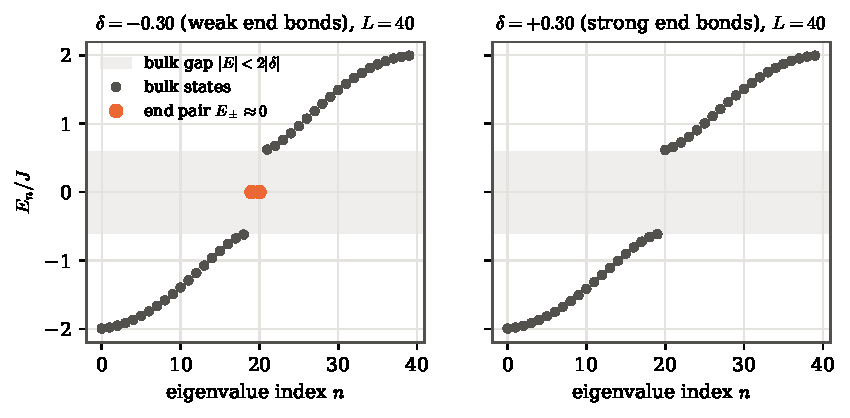
\includegraphics[width=\textwidth]{step1_spectrum.pdf}
  \caption{One-particle spectra, $L=40$.
  For weak end bonds ($\delta=-0.30$, left), two levels sit at $E\approx0$ inside the bulk gap.
  Reversing $\delta$ (right) removes them and leaves the bulk bands unchanged.}
  \label{fig:spectrum}
\end{figure}

\begin{figure}[t]
  \centering
  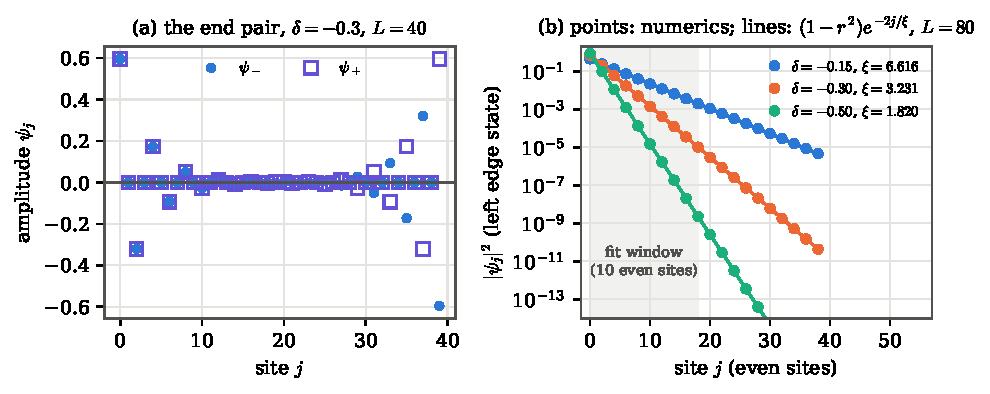
\includegraphics[width=\textwidth]{step1_edge_states.pdf}
  \caption{(a) The two eigenstates nearest zero ($\delta=-0.30$, $L=40$) are bonding and antibonding combinations of the two ends.
  (b) The left-edge state for $L=80$ (points) against Eq.~\eqref{eq:xi} with no free parameters (lines).
  The shading marks the fit window.}
  \label{fig:edge}
\end{figure}

\paragraph{Edge state and localisation length.}
For every $\delta<0$ there are exactly two levels with $|E|<|\delta|$, and for every $\delta>0$ there are none (Fig.~\ref{fig:spectrum}).
The left-edge state agrees with Eq.~\eqref{eq:xi} over fourteen decades, and its odd-site weight is below $10^{-28}$ (Fig.~\ref{fig:edge}).
The $X$ and $\Gamma$ constructions give the same state to $6\times10^{-15}$.
Table~\ref{tab:xi} lists the fitted lengths.
At $\delta=-0.30$ the fit reproduces $\xi = 3.230813126$ to $10^{-15}$ for $L\ge80$.

The one visible deviation is $3.7\times10^{-4}$, at $\delta=-0.15$, $L=40$, where $L/\xi = 6$.
It grows with $n_{\rm fit}$, so it comes from the opposite edge and not from the fit.
The finite-chain state obeys $h\psi^L = \pm\varepsilon_0\psi^R$, which perturbs the recursion at relative order $(1-r^2)\,r^{L-2\ell-2}$.
This estimate gives about $10^{-4}$ to $10^{-3}$ across the fit window, matching the observed deviation.
It falls rapidly with $L$: at the same $\delta$ it is $2\times10^{-9}$ at $L=80$ and $1\times10^{-14}$ at $L=120$.

\begin{table}[t]
  \centering
  \footnotesize
  \setlength{\tabcolsep}{4.5pt}
  \begin{tabular}{rrcccccc}
    \toprule
    $\delta$ & $L$ & $\xi_{\rm fit}$ ($n_{\rm fit}=10$) &
    \multicolumn{3}{c}{$(\xi_{\rm fit}-\xi)/\xi$ for $n_{\rm fit} = 6,\ 8,\ 10$} &
    $\Delta E$ (exact) & resolved by \texttt{eigh}? \\
    \midrule
    $-0.15$ & 40  & 6.613912628 & $-6.0\times10^{-5}$  & $-1.5\times10^{-4}$  & $-3.7\times10^{-4}$  & $2.4713\times10^{-3}$  & yes \\
    $-0.15$ & 80  & 6.616363065 & $-3.4\times10^{-10}$ & $-8.3\times10^{-10}$ & $-2.1\times10^{-9}$  & $5.8523\times10^{-6}$  & yes \\
    $-0.15$ & 120 & 6.616363079 & $-1.5\times10^{-15}$ & $-4.8\times10^{-15}$ & $-1.2\times10^{-14}$ & $1.3860\times10^{-8}$  & yes \\
    \midrule
    $-0.30$ & 40  & 3.230812682 & $-2.3\times10^{-9}$  & $-1.7\times10^{-8}$  & $-1.4\times10^{-7}$  & $7.7511\times10^{-6}$  & yes \\
    $-0.30$ & 80  & 3.230813126 & $0$                  & $1.6\times10^{-15}$  & $2.6\times10^{-15}$  & $3.2543\times10^{-11}$ & yes \\
    $-0.30$ & 120 & 3.230813126 & $1.4\times10^{-15}$  & $1.4\times10^{-16}$  & $-4.1\times10^{-16}$ & $1.3663\times10^{-16}$ & no \\
    \midrule
    $-0.50$ & 40  & 1.820478453 & $-2.4\times10^{-16}$ & $-3.2\times10^{-14}$ & $-1.7\times10^{-12}$ & $7.6479\times10^{-10}$ & yes \\
    $-0.50$ & 80  & 1.820478453 & $3.7\times10^{-16}$  & $2.4\times10^{-16}$  & $2.4\times10^{-16}$  & $2.1934\times10^{-19}$ & no \\
    $-0.50$ & 120 & 1.820478453 & $0$                  & $-2.4\times10^{-16}$ & $0$                  & $6.2906\times10^{-29}$ & no \\
    \bottomrule
  \end{tabular}
  \caption{Fitted localisation length and end-pair splitting.
  Exact values: $\xi = 6.616363079$, $3.230813126$, $1.820478453$ for $|\delta| = 0.15,\,0.30,\,0.50$.
  $\Delta E$ (exact) is from the 80-digit Sturm bisection.
  ``Resolved'' means dense diagonalisation agrees with it to $10^{-6}$.}
  \label{tab:xi}
\end{table}

\begin{figure}[t]
  \centering
  \begin{minipage}{0.49\textwidth}\centering
    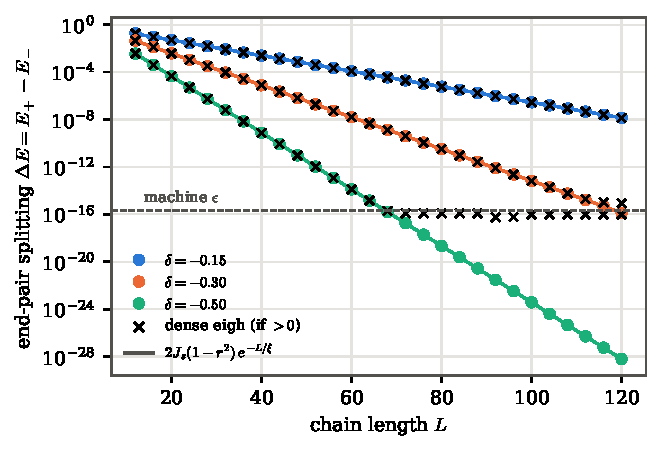
\includegraphics[width=\textwidth]{step1_splitting.pdf}
  \end{minipage}\hfill
  \begin{minipage}{0.49\textwidth}\centering
    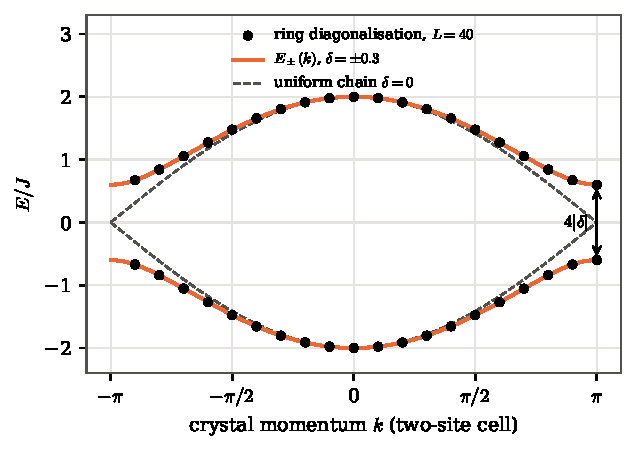
\includegraphics[width=\textwidth]{step1_ring_bands.pdf}
  \end{minipage}
  \caption{Left: end-pair splitting against $L$.
  Circles are exact (80-digit) values, lines are Eq.~\eqref{eq:splitting}, and crosses are dense diagonalisation, which stops at a round-off floor near $10^{-16}$.
  Right: ring spectrum, $L=40$, $\delta=-0.30$ (points), against $E_\pm(k)$ (line); the uniform chain is dashed.}
  \label{fig:split}
\end{figure}

\paragraph{Splitting.}
The splitting falls monotonically with $L$ (Fig.~\ref{fig:split}, left).
Fitting $\ln\Delta E$ against $L$ for $L\ge40$ gives slopes $-0.151141$, $-0.309520$ and $-0.549306$.
The predicted values $-1/\xi$ are $-0.151140$, $-0.309520$ and $-0.549306$.
The full formula, Eq.~\eqref{eq:splitting}, agrees with the exact values to within $5\times10^{-5}$ at $L=40$, and to round-off for $L\ge80$.
Dense diagonalisation cannot resolve splittings below about $10^{-15}$, so it fails at three grid points (Table~\ref{tab:xi}).

\paragraph{Ring.}
The ring spectrum matches Eq.~\eqref{eq:bands} to $5\times10^{-15}$ for every $L$ and $\delta$.
The gap is $4|\delta|$ and the bulk addition cost is $2|\delta|$, both to $2\times10^{-15}$.
The spectra for $+\delta$ and $-\delta$ are identical (Fig.~\ref{fig:split}, right).
On the odd-$M$ rings $L=10,14,18$ the spectrum also matches Eq.~\eqref{eq:bands}, and the gap equals $2\min_k E_+(k)$ over the allowed $k$, both to $2\times10^{-15}$.

\paragraph{Choosing the half-filled ground state.}
At half filling exactly one of the end pair is occupied.
Where the splitting is unresolved, the eigensolver returns $\psi^L$ and $\psi^R$ in arbitrary order, so ``fill the lowest $N$ orbitals'' becomes ill-defined.
At $L=120$, $\delta=-0.5$, filling the wrong state moves $\langle n_0\rangle$ away from $\tfrac12$ by order one.
In that case the numerically computed $t$ also has the wrong sign.
We therefore fix the convention analytically: fill the bonding orbital
\begin{equation}
  \phi_- = \tfrac{1}{\sqrt2}\big(\psi^L - s\,\psi^R\big),\qquad s = \operatorname{sgn}t = (-1)^{L/2},
  \label{eq:convention}
\end{equation}
with $\psi^L_0>0$ and $\psi^R_{L-1}>0$.
The numerical sign of $t$ agrees with $(-1)^{L/2}$ at every point where the splitting is resolved, for both even $L/2$ (the grid) and odd $L/2$ ($L=18,42,62,82$).
With this convention, $\langle n_0\rangle = \tfrac12$ to $10^{-15}$ on every grid point.
The edge addition weight is then $z_0 = |\phi_+(0)|^2/(1-\langle n_0\rangle) = |\psi^L_0|^2$ to round-off, and $z_0$ agrees with $1-r^2$ to $4\times10^{-5}$.

\begin{table}[h]
  \centering
  \footnotesize
  \begin{tabular}{p{11.2cm}l}
    \toprule
    Check (all $L$ and $\delta$) & largest deviation \\
    \midrule
    $J_0 = \Jw$ and $J_{L-2} = J_0$ for $\delta<0$; $h$ symmetric & exact \\
    Spectrum symmetric under $E\to-E$ & $2.4\times10^{-15}$ \\
    Truncated zero mode: $h\psi = 0$ except the last row, $(h\psi)_{L-1} = -\Jw\psi_{L-2}$ & $5.6\times10^{-17}$ \\
    Two in-gap states for $\delta<0$, none for $\delta>0$; $\min|E|\ge2|\delta|$ for $\delta>0$ & exact \\
    Fitted $\xi$ against Eq.~\eqref{eq:xi} (tolerance $10^{-3}$) & $3.7\times10^{-4}$ \\
    Left state: weight on odd sites; $X$ and $\Gamma$ constructions agree & $2.4\times10^{-29}$; $5.8\times10^{-15}$ \\
    Slope of $\ln\Delta E$ against $L$ equals $-1/\xi$ (relative) & $1.5\times10^{-6}$ \\
    Eq.~\eqref{eq:splitting} against exact splitting, $L\ge40$ (relative) & $4.8\times10^{-5}$ \\
    Ring: spectrum $=E_\pm(k)$, gap $=4|\delta|$, addition cost $=2|\delta|$, $\pm\delta$ identical & $4.9\times10^{-15}$ \\
    $\operatorname{sgn}t = (-1)^{L/2}$ where resolved; $\langle n_0\rangle = \tfrac12$; $z_0 = |\psi^L_0|^2$ & $1.0\times10^{-15}$ \\
    Odd $L/2$ ($L=18,42,62,82$): $\operatorname{sgn}t = -1$ and bonding below antibonding where resolved; $\langle n_0\rangle = \tfrac12$; $z_0 = |\psi^L_0|^2$ & $1.0\times10^{-15}$ \\
    Odd $L/2$: Eq.~\eqref{eq:splitting} against exact splitting, $L\ge40$ (relative) & $2.8\times10^{-5}$ \\
    Odd-$M$ rings ($L=10,14,18$): spectrum $=E_\pm(k)$; gap $=2\min_k E_+(k) > 4|\delta|$ & $2.2\times10^{-15}$ \\
    \bottomrule
  \end{tabular}
  \caption{Step 1 validation: 37 checks in the notebook, all passed.}
  \label{tab:checks1}
\end{table}

%----------------------------------------------------------------------
\subsection{Conclusion}

The free edge problem is solved and verified.
\begin{itemize}
  \item The edge state is the analytic zero mode, Eq.~\eqref{eq:xi}, to round-off once $L/\xi\gtrsim25$.
  At smaller $L/\xi$ the only correction comes from the opposite edge, and its size is predicted.
  \item The end pair splits by $2\Js(1-r^2)e^{-L/\xi}$, with slope and prefactor both confirmed.
  \item Reversing $\delta$ removes the end pair while leaving the bulk spectrum unchanged.
  The edge state is therefore a property of how the bulk is terminated, not of the bulk energies.
\end{itemize}
Two results carry into the interacting problem.
First, once the splitting drops below round-off, the half-filled ground state must be selected by an explicit rule, Eq.~\eqref{eq:convention}; otherwise edge observables change at order one.
Second, the many-body calculation must reproduce the $V=0$ values $\langle n_j\rangle = \tfrac12$, $z_0 = 1-r^2$ and $\xi_W = \xi$, with bulk addition threshold $\Delta_+ = 2|\delta|$ on rings with $L$ divisible by 4 and half the larger gap above on odd-$M$ rings.

%======================================================================
\section{Step 2: a many-body calculation we can trust}
\label{sec:step2}

\subsection{What was done}

At $V\neq0$ the problem no longer reduces to an $L\times L$ matrix.
Every hopping term contains one $c\dg$ and one $c$, so $[H,\hat N]=0$, and $H$ splits into sectors of dimension $\binom{L}{N}$, which is $12\,870$ at $L=16$ and $48\,620$ at $L=18$.
We store an occupation state as the integer $s=\sum_j n_j2^j$ and build separate sparse matrices in the sectors $N=L/2$ and $N=L/2\pm1$.
For $L=6,8,10$ we diagonalise the whole matrix.
For $L\ge12$ we find the lowest levels with a Lanczos solver (\texttt{eigsh} with \texttt{tol=0}, a fixed seed and at least 40 Lanczos vectors).

We ran the open chain at $L=8$ first and then at $L=12,16,18$, with $\delta=\pm0.30$ and $V=0,0.5,1,2,3$.
Each point also has a ring at the same $(L,\delta,V)$, which gives the bulk addition threshold $\Delta_+=E_{0,\rm ring}^{N+1}-E_{0,\rm ring}^{N}$ needed in Step~3.
We refined an interval of $V$ in steps of $0.25$ if the symmetry labels of the two lowest levels changed, if a gap stopped being monotonic in $V$ or changed its trend with $L$, or if the overlap of neighbouring ground states fell below $0.99$.
On the coarse grid this flagged every interval except $0\le V\le0.5$ at $\delta=+0.30$.
The sizes $L=10,14$ were added on the coarse grid to compare sizes with the same parity of $M=L/2$.
Energies, residuals, labels and solver settings for every level are saved in \texttt{data/}.

\paragraph{Sign rule.}
We fix the operator order and read off the action of $c_j\dg$:
\begin{equation}
  |n\rangle = (c_0\dg)^{n_0}\cdots(c_{L-1}\dg)^{n_{L-1}}|0\rangle,
  \qquad
  c_j\dg|n\rangle = (-1)^{\sum_{l<j}n_l}\,(1-n_j)\,|n+e_j\rangle .
\end{equation}
For $c_a\dg c_b$ we annihilate at $b$ first and then create at $a$, evaluating the second sign on the intermediate state.
On an open-chain bond the two strings cancel, so every off-diagonal element of $H$ is exactly $-J_j$.
On a ring, the hop across the closing bond moves a particle past the other $N-1$, so it carries the sign $(-1)^{N-1}$.
With this order, the Jordan--Wigner map $c_j=\big(\prod_{l<j}Z_l\big)|0\rangle\langle1|_j$, $n_j=(1-Z_j)/2$ sends the occupation basis to the computational basis with no extra signs, and
\begin{equation}
  H = -\frac12\sum_j J_j\left(X_jX_{j+1}+Y_jY_{j+1}\right) + \frac V4\sum_j Z_jZ_{j+1} .
  \label{eq:jw}
\end{equation}
The closing bond of a ring becomes $-\tfrac12J_{L-1}(X_0X_{L-1}+Y_0Y_{L-1})\prod_{0<l<L-1}Z_l$, whose parity string equals $(-1)^{N-1}$ in sector $N$.
Fermion signs therefore enter only through $\langle c_i\dg c_j\rangle$ with $|i-j|\ge2$, through the operators $c_j$ and $c_j\dg$, and through the closing bond.
A spin-chain code with no strings would reproduce every open-chain energy, so these three places have their own tests, each with a negative control.

\paragraph{Symmetries.}
The particle--hole map $C$: $c_j\to(-1)^jc_j\dg$ preserves every term of Eq.~\eqref{eq:H}, sends $n_j\to1-n_j$ and maps $N\to L-N$; it is the bit complement with sign $+1$.
So the spectra in sectors $N\pm1$ are identical at every $V$, and the addition and removal gaps are equal.
The reflection $R$: $c_j\to c_{L-1-j}$ commutes with $H$ because $J_{L-2-j}=J_j$; it is the bit reversal times $(-1)^{N(N-1)/2}$, the sign of reordering $N$ creation operators.
On a ring, translation by one site maps $\delta\to-\delta$, so ring spectra are identical for $\pm\delta$ at every $V$.

\paragraph{Choosing the half-filled ground state.}
On the open chain all off-diagonal elements in a sector are $-J_j<0$, and any configuration can reach any other by hops.
The Perron--Frobenius theorem then says that the lowest level is non-degenerate, with a strictly positive eigenvector, at every $V$ and $\delta$.
$C$ and bit reversal map positive vectors to positive vectors, so the ground state always has
\begin{equation}
  C=+1,\qquad R=(-1)^{N(N-1)/2},\qquad \langle n_j\rangle=\tfrac12 .
  \label{eq:pf}
\end{equation}
This generalises the rule of Eq.~\eqref{eq:convention}.
We take the lowest eigenvector with $\sum_s\psi_s>0$ and verify Eq.~\eqref{eq:pf} and positivity.
If the neutral gap $E_1^N-E_0^N$ falls below $\eta=10^{-8}$, the eigenvector order cannot be trusted, so we diagonalise $C$ inside the cluster and keep the $C=+1$ vector, and the code raises an error if that does not fix the state.
At $V=0$ this is the bonding state of Eq.~\eqref{eq:convention}, which we confirm through the correlation matrix.
On the present grid the cluster branch is never used, because the smallest neutral gap is $4.3\times10^{-3}$ ($L=18$, $V=3$).
It is needed for the larger chains of Step~7, so we tested it on a constructed pair.

%----------------------------------------------------------------------
\subsection{Results and verification}

\begin{figure}[t]
  \centering
  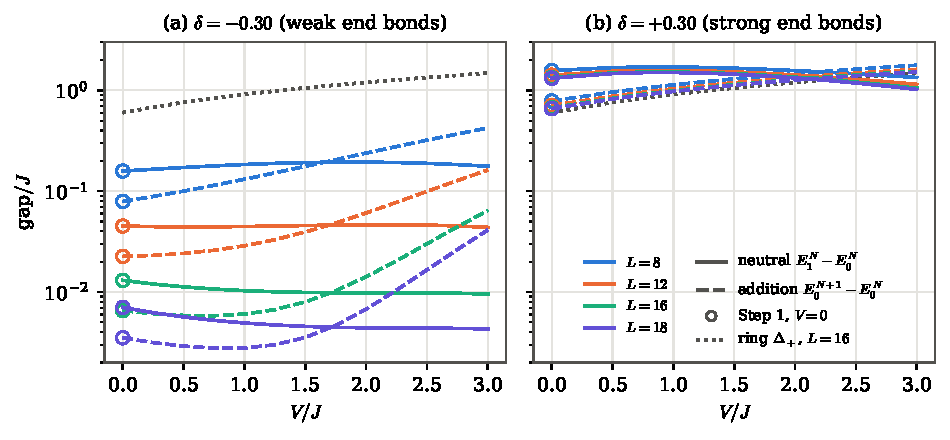
\includegraphics[width=\textwidth]{step2_gaps.pdf}
  \caption{Neutral gap (solid) and addition gap (dashed) on the open chain against $V$.
  Open circles are the Step~1 values at $V=0$, computed from the hopping matrix alone.
  The dotted line is the ring threshold $\Delta_+$ at $L=16$.
  For $\delta=-0.30$ both gaps fall with $L$ and stay far below $\Delta_+$.
  For $\delta=+0.30$ the addition gap sits just above $\Delta_+$.}
  \label{fig:gaps}
\end{figure}

\begin{table}[t]
  \centering
  \footnotesize
  \setlength{\tabcolsep}{3.5pt}
  \begin{tabular}{rr*{8}{l}l}
    \toprule
    & & \multicolumn{2}{c}{$L=8$} & \multicolumn{2}{c}{$L=12$} & \multicolumn{2}{c}{$L=16$} & \multicolumn{2}{c}{$L=18$} & \\
    $\delta$ & $V$ & neutral & add. & neutral & add. & neutral & add. & neutral & add. & $\Delta_+$ \\
    \midrule
    $-0.30$ & 0 & 0.158 & 0.0791 & 0.0451 & 0.0226 & 0.0131 & 0.00653 & 0.00703 & 0.00351 & 0.6000 \\
    $-0.30$ & 0.5 & 0.172 & 0.100 & 0.0442 & 0.0241 & 0.0112 & 0.00586 & 0.00566 & 0.00291 & 0.7585 \\
    $-0.30$ & 1 & 0.184 & 0.131 & 0.0446 & 0.0288 & 0.0103 & 0.00605 & 0.00493 & 0.00279 & 0.9106 \\
    $-0.30$ & 2 & 0.194 & 0.238 & 0.0464 & 0.0608 & 0.00980 & 0.0142 & 0.00441 & 0.00675 & 1.1969 \\
    $-0.30$ & 3 & 0.177 & 0.423 & 0.0437 & 0.162 & 0.00954 & 0.0644 & 0.00431 & 0.0412 & 1.4806 \\
    \midrule
    $+0.30$ & 0 & 1.57 & 0.783 & 1.41 & 0.706 & 1.34 & 0.670 & 1.32 & 0.658 & 0.6000 \\
    $+0.30$ & 0.5 & 1.68 & 0.960 & 1.54 & 0.873 & 1.48 & 0.832 & 1.47 & 0.820 & 0.7585 \\
    $+0.30$ & 1 & 1.70 & 1.13 & 1.57 & 1.03 & 1.52 & 0.989 & 1.50 & 0.975 & 0.9106 \\
    $+0.30$ & 2 & 1.57 & 1.46 & 1.42 & 1.34 & 1.35 & 1.28 & 1.33 & 1.26 & 1.1969 \\
    $+0.30$ & 3 & 1.34 & 1.77 & 1.15 & 1.61 & 1.05 & 1.54 & 1.02 & 1.52 & 1.4806 \\
    \bottomrule
  \end{tabular}
  \caption{Neutral gap $E_1^N-E_0^N$ and addition gap $E_0^{N+1}-E_0^N$ on the open chain, and the ring threshold $\Delta_+$ at $L=16$, which is identical for $\pm\delta$.}
  \label{tab:gaps}
\end{table}

\begin{table}[t]
  \centering
  \footnotesize
  \begin{tabular}{rrcccc}
    \toprule
    $\delta$ & $V$ & $L=8$ & $L=12$ & $L=16$ & $L=18$ \\
    \midrule
    $-0.30$ & 0 & $-4.55115091$ & $-7.29433511$ & $-10.07124071$ & $-11.46436524$ \\
    $-0.30$ & 1 & $-5.38330812$ & $-8.59361995$ & $-11.86317538$ & $-13.50473059$ \\
    $-0.30$ & 2 & $-6.38674876$ & $-10.11768108$ & $-13.93086953$ & $-15.84831685$ \\
    $-0.30$ & 3 & $-7.55692209$ & $-11.88617401$ & $-16.29398502$ & $-18.51120790$ \\
    \midrule
    $+0.30$ & 0 & $-5.48423862$ & $-8.27637905$ & $-11.06853533$ & $-12.46461383$ \\
    $+0.30$ & 1 & $-6.47951089$ & $-9.76851518$ & $-13.05753117$ & $-14.70203936$ \\
    $+0.30$ & 2 & $-7.56148113$ & $-11.40639098$ & $-15.25132360$ & $-17.17379035$ \\
    $+0.30$ & 3 & $-8.72472182$ & $-13.18286330$ & $-17.64115537$ & $-19.87030841$ \\
    \midrule
    \multicolumn{2}{r}{worst residual} & $1.4\times10^{-14}$ & $7.0\times10^{-14}$ & $9.0\times10^{-14}$ & $1.3\times10^{-13}$ \\
    \bottomrule
  \end{tabular}
  \caption{Half-filled ground-state energy $E_0^N$ on the open chain.
  The worst residual covers all recorded levels in $N$ and $N\pm1$ at that size.
  At every point the ground state has $C=+1$, $R=(-1)^{N(N-1)/2}$ and level 1 has $C=-1$ and the opposite $R$.}
  \label{tab:e0}
\end{table}

\paragraph{Gaps.}
Figure~\ref{fig:gaps} and Table~\ref{tab:gaps} give the main result.
At $V=0$ every curve starts on its Step~1 value.
For $\delta=-0.30$ both gaps fall with $L$ at every $V$, and at $L=16$ the addition gap stays below $5\%$ of $\Delta_+$.
For $\delta=+0.30$ there is no low-energy pair: the neutral gap stays above 1, and at $L=16$ the addition gap lies $0.06$ to $0.08$ above $\Delta_+$.
So reversing $\delta$ still removes the low-energy pair at every $V\le3$ on this grid.

The labels in Eq.~\eqref{eq:pf} hold at every point of the grid, and level 1 keeps $C=-1$ and the opposite $R$ (Table~\ref{tab:e0}), so no crossing involves the two lowest levels.
Levels 2 to 5 do cross, but they stay at least $0.7$ above the ground state.
On the refined grid neighbouring ground states overlap by at least $0.996$, and the only remaining trigger is a smooth extremum of a gap, for example the maximum of the $\delta=+0.30$ neutral gap near $V=1$ at every $L$.
Nothing singles out $V=2$ at these sizes, in line with $V=2$ being the transition of the uniform chain only.

\paragraph{Is the matrix correct?}
$H=H_{\rm hop}(\delta)+VH_{\rm int}$ is linear in $V$, and $H_{\rm int}$ does not depend on $\delta$.
So it is enough to test $H_{\rm hop}$ at $V=0$ and $H_{\rm int}$ at some $V\neq0$.

At $V=0$ every many-body level must be a sum of $N$ one-particle energies.
This holds for the whole spectrum at $L=6,8,10$, open and ring, and for the lowest levels with their exact multiplicities up to $L=18$.
The neutral and addition gaps reproduce the 80-digit splitting $\Delta E$ and $\Delta E/2$ of Step~1, and $\langle c_i\dg c_j\rangle$ reproduces the filled-orbital matrix built on the bonding orbital of Eq.~\eqref{eq:convention}, at $L=6$ to $18$.

At $V\neq0$ we have five routes that do not rest on the $V=0$ checks.
First, we verify $\{c_i,c_j\dg\}=\delta_{ij}$ and $\{c_i,c_j\}=0$ directly, and then $H$ written as a literal product of these operators equals the sparse matrix, as does the Jordan--Wigner form, Eq.~\eqref{eq:jw}, on all $2^L$ states.
Second, $L=2$ and $L=4$ can be solved by hand.
With $a=J_0$ and $b=J_1$, the ring at $L=4$, $N=2$ has the spectrum $\{0,\,0,\,-V/2\pm\sqrt{V^2/4+4a^2},\,-V/2\pm\sqrt{V^2/4+4b^2}\}$, which depends on the closing sign $-1$.
Third, first-order perturbation theory with Wick's theorem predicts $dE/dV$ at $V=0$ for $E_0^N$, $E_1^N$ and $E_0^{N+1}$ from the Step~1 orbitals alone.
Fourth, at large $V$ the ground states are the two charge-density waves, and an added particle makes one mobile doubly occupied bond, so to leading orders
\begin{gather}
  E_0^N = -\frac{(L-1)V}{4} - \frac1V\Big[\sum_{j=1}^{L-3}J_j^2+2\big(J_0^2+J_{L-2}^2\big)\Big] + O(V^{-3}),
  \\
  E_0^{N+1}-E_0^N = \frac V2 - 2(1-\delta)\cos\frac{\pi}{M+1} + O(V^{-1}).
\end{gather}
The errors shrink by the predicted factors of 8 and 2 when $V$ doubles from 200 to 400.
Fifth, at $\delta=0$ a sublattice rotation gives $H=2H_{\rm XXZ}(\Delta=V/2)$, which is integrable.
Solving the Bethe equations~\cite{alcaraz} shares no code with the matrix construction, and it agrees with exact diagonalisation to $7\times10^{-14}$ for $V=0.5$ to 2 up to $L=18$, on open chains and on odd-$N$ rings.
At $V=2$ the energy per site approaches Hulth\'en's $2(\tfrac14-\ln2)$~\cite{hulthen}.

\paragraph{Are the eigenpairs right?}
All residuals are below $7\times10^{-14}$ at $L\le10$ and below $7\times10^{-13}$ in production, well inside the targets $10^{-10}$ and $10^{-9}$.
Lanczos agrees with dense diagonalisation at $L=12$, and the eigenvalue agrees with an independent $\langle\psi|H|\psi\rangle$ built from correlators without using the matrix.

A small residual does not make every observable equally accurate, because a residual $\|r\|$ only bounds the eigenvector error by $\|r\|/\mathrm{gap}$, and an observable can shift by up to $2\|r\|/\mathrm{gap}$.
For $\delta<0$ the nearest level is the end partner.
At $L=18$, $V=0$, the raw Lanczos correlators deviate from Step~1 by $1.2\times10^{-12}$, inside the bound $4.8\times10^{-12}$.
The partner has $C=-1$, so projecting onto $C=+1$ must remove the error, and it does: the deviation drops to $2\times10^{-15}$.
The same limit will matter in later steps wherever the gap is small.

\paragraph{Can the checks fail?}
Three negative controls are built in.
Without the closing sign the ring energies fail for every even $N$ (by at least $0.061$) and for no odd $N$.
Without the string, $\langle c_i\dg c_j\rangle$ stays correct for adjacent sites but is off by up to $0.68$ beyond them.
An unselected equal mixture of the end pair moves $\langle n_0\rangle$ away from $\tfrac12$ by $0.38$ at $L=12$, $V=1$.
We also broke the code on purpose in 16 ways (\texttt{checks/step2\_mutation\_test.py}).
Fifteen were caught.
The other, reversing the bit order in Jordan--Wigner, leaves the matrix unchanged to $2\times10^{-16}$ because $H$ is reflection symmetric, so it is not an error for this model.

\begin{table}[t]
  \centering
  \footnotesize
  \begin{tabular}{p{10.2cm}l}
    \toprule
    Check & largest deviation \\
    \midrule
    $H$ symmetric; number conserved; sector sizes $\binom{L}{N}$; $\{c_i,c_j\dg\}=\delta_{ij}$; $H$ = literal operator product & exact \\
    Jordan--Wigner fixed-$N$ blocks, all $N$, open and ring; full spectrum & exact; $4.9\times10^{-14}$ \\
    $V=0$: whole spectrum, $L\le10$; lowest levels with multiplicities, $L\le18$ & $3.6\times10^{-14}$; $6.2\times10^{-14}$ \\
    $V=0$: $\langle c_i\dg c_j\rangle$, $L\le18$, $C$-projected; raw vector within bound & $2.0\times10^{-15}$; ratio $0.23$ \\
    $V=0$: gaps against 80-digit $\Delta E$; addition weights against the empty orbital & $4.8\times10^{-14}$; $6.4\times10^{-14}$ \\
    Sum rule $\sum_mw_{jm}=1-\langle n_j\rangle$, whole $N+1$ spectrum, every $V$ & $2.2\times10^{-15}$ \\
    Ring, $V=0$: $E_0$ for all $N$; $\Delta_+$ for even and odd $M$ & $4.4\times10^{-15}$; $3.7\times10^{-14}$ \\
    Operator maps of $C$ and $R$; spectrum$(N+1)=$ spectrum$(N-1)$; $[C,H]=[R,H]=0$ & exact; $3.6\times10^{-14}$; $3.6\times10^{-15}$ \\
    Ring spectra for $\pm\delta$; $R$ of $\Omega_N$ against orbital parities at $V=0$ & $6.3\times10^{-14}$; $4.9\times10^{-15}$ \\
    $L=2$, and $L=4$ open and ring, against closed forms, every $V$ & $7.1\times10^{-15}$ \\
    Weak coupling: $dE/dV$ against Wick (error $O(\text{step}^2)$) & $4.1\times10^{-8}$ \\
    Strong coupling at $V=400$: $E_0^N$; addition gap (errors scale as predicted) & $3.0\times10^{-6}$; $6.4\times10^{-3}$ \\
    Bethe ansatz, $\delta=0$: open chain; odd-$N$ ring & $6.2\times10^{-14}$; $6.8\times10^{-14}$ \\
    Hulth\'en energy per site from $L=16,18$ (finite size, tolerance $2\times10^{-3}$) & $1.0\times10^{-3}$ \\
    Residuals: all eigenpairs $L\le10$; production open; production ring & $7.0\times10^{-14}$; $1.3\times10^{-13}$; $6.1\times10^{-13}$ \\
    Lanczos against dense, $L=12$; against another seed, $L=16$ & $7.1\times10^{-14}$; $8.7\times10^{-14}$ \\
    Eigenvalue against independent $\langle H\rangle$, whole grid & $7.8\times10^{-14}$ \\
    Whole grid: $\min_s\psi_s/\max_s\psi_s$; $C$, $R$ labels; $\langle n_j\rangle=\tfrac12$ & $-8.9\times10^{-16}$; exact; $4.2\times10^{-12}$ \\
    State selection: rotated pair recovered; raises when $C$ does not fix the state & $1.2\times10^{-14}$; exact \\
    \bottomrule
  \end{tabular}
  \caption{Step 2 validation: 61 checks in the notebook, all passed.
  Deviations are from the run saved in \texttt{data/step2\_checks.csv}; round-off values change slightly between runs.}
  \label{tab:checks2}
\end{table}

\begin{table}[t]
  \centering
  \footnotesize
  \begin{tabular}{lcccccc}
    \toprule
    & sizes & $V=0$ & $0.5$ & $1$ & $2$ & $3$ \\
    \midrule
    neutral gap & 12, 16 & 3.23 & 2.92 & 2.73 & 2.57 & 2.63 \\
    & 14, 18 & 3.23 & 2.92 & 2.72 & 2.52 & 2.55 \\
    addition gap & 12, 16 & 3.23 & 2.83 & 2.57 & 2.75 & 4.34 \\
    & 14, 18 & 3.23 & 2.84 & 2.57 & 2.71 & 4.43 \\
    $U_{\rm eff}$ & 12, 16 & -- & 1.87 & 2.03 & 2.86 & 4.68 \\
    & 14, 18 & -- & 1.82 & 1.98 & 2.83 & 4.71 \\
    \bottomrule
  \end{tabular}
  \caption{Two-size decay lengths $(L_2-L_1)/\ln[\mathrm{gap}(L_1)/\mathrm{gap}(L_2)]$ at $\delta=-0.30$, from pairs of sizes with the same parity of $M$.
  Step~1 gives $\xi=3.2308$ at $V=0$.
  These are finite-size estimates, not converged lengths.}
  \label{tab:lengths}
\end{table}

%----------------------------------------------------------------------
\subsection{Conclusion}

The many-body calculation is verified for $L\le18$ on this grid.
\begin{itemize}
  \item The matrices are Eq.~\eqref{eq:H} in sectors $N$ and $N\pm1$, including the fermion sign on a ring's closing bond.
  They reproduce Step~1 at $V=0$, and closed forms, both perturbative limits and the Bethe ansatz at $V\neq0$.
  \item The half-filled ground state is unique on the open chain, with labels fixed by Eq.~\eqref{eq:pf}.
  \item On this grid, both gaps at $\delta=-0.30$ fall with $L$ and stay well below the ring threshold, while $\delta=+0.30$ has no low-energy pair.
  No crossing involves the two lowest levels, and $V=2$ shows no special feature.
\end{itemize}
Step~3 inherits $\Omega_N$, the operators $c_j\dg$, the ring thresholds and two observations, which are hypotheses and not results.

First, the two gaps stop being controlled by one length (Table~\ref{tab:lengths}).
Two end modes with symmetries $C$ and $R$ have the general form $t(a_L\dg a_R+\text{h.c.})+U(n_L-\tfrac12)(n_R-\tfrac12)$, which gives a neutral gap $2|t|$ and an addition gap $|t|+U/2$.
This suggests reading $U_{\rm eff}=2(E_0^{N+1}-E_0^N)-(E_1^N-E_0^N)$ as an effective repulsion between the ends.
It vanishes at $V=0$ to $8\times10^{-14}$ and is $0.078$ at $L=18$, $V=3$, where the next levels in sectors $N$ and $N+1$ lie about $1.15$ higher.
Its two-size length grows from about $1.8$ at $V=0.5$ to about $4.7$ at $V=3$.
At $V=3$ it changes by $0.13$ between the size pairs $(8,12)$ and $(16,18)$, while the addition-gap length changes by $0.31$ and is still rising.
Whether the end state itself has changed is a separate question, which energies cannot answer and $z_0$ and $\xi_W$ can.

Second, the edge window may not stay isolated at strong repulsion.
At $V=3$ the second addition level lies at $\omega=1.26$ for $L=16$ and $1.18$ for $L=18$, against $0.8\Delta_+=1.18$ on the $L=16$ ring and $1.24$ on the $L=18$ ring.
So it is just outside the window at $L=16$ and inside it at $L=18$.
Step~3 must test this window directly and report it if no isolated window exists.

% \section{Step 3: localisation and coherence}
% \section{Step 4: dynamics of an added edge particle}
% \section{Step 5: entropy resolved by particle number}
% \section{Step 6: bulk polarisation and the competing ordered state}
% \section{Step 7: larger chains with MPS}
% \section{Step 8: extension}
% \section{Conclusions and limits}

%======================================================================
\begin{thebibliography}{9}
\bibitem{monkman}
K.~Monkman and J.~Sirker, \emph{Operational entanglement of symmetry-protected topological edge states}, \href{https://arxiv.org/abs/2005.13026}{arXiv:2005.13026}.
\bibitem{vidal}
G.~Vidal, \emph{Efficient simulation of one-dimensional quantum many-body systems}, \href{https://arxiv.org/abs/quant-ph/0310089}{arXiv:quant-ph/0310089}.
\bibitem{alcaraz}
F.~C.~Alcaraz, M.~N.~Barber, M.~T.~Batchelor, R.~J.~Baxter and G.~R.~W.~Quispel, \emph{Surface exponents of the quantum XXZ, Ashkin--Teller and Potts models}, J.~Phys.~A \textbf{20}, 6397 (1987).
\bibitem{hulthen}
L.~Hulth\'en, \emph{\"Uber das Austauschproblem eines Kristalles}, Ark.~Mat.~Astron.~Fys.~\textbf{26A}, 1 (1938).
\end{thebibliography}

\end{document}
